\section{Theorie}

\subsection{Zielsetzung}

In dem folgenden Versuch sollen mehrere Gesetzmäßigkeiten der geometrischen Optik,
wie zum Beispiel das Abbildungsgesetz und die Linsengleichung, mit verschiedenen
Versuchsaufbauten überprüft werden. Zudem sollen diese dann genutzt werden, um
für verschiedene Linsen(-Systeme) die Brennweite zu bestimmen.

\subsection{Grundlagen der geometrischen Optik}

Grundlegend werden in der Optik Linsen aus verschiedenen Materialien betrachtet,
die optisch dichter sind als Licht. Durch diese Eigenschaft werden Lichtstrahlen
bei Durchgang solch eines Mediums nach dem Brechungsgesetz gebrochen. Da die
auftretende Brechung auch Abhängig von der Geometrie des Körpers ist, werden
die Linsen meist in zwei Kategorien eingeteilt. Ein Typus ist die Sammellinse, bei
der parallel einfallende Lichtstrahlen zum Einfallslot hin gebrochen werden.
Dadurch entsteht an dem Punkt, an dem sich die Lichtstrahlen bündeln ein reeles
Bild in der Entfernung b (Bildweite) zur Hauptebene der Linse (siehe Abbildung
\ref{fig:Sammellinse}).

\begin{figure}
  \centering
  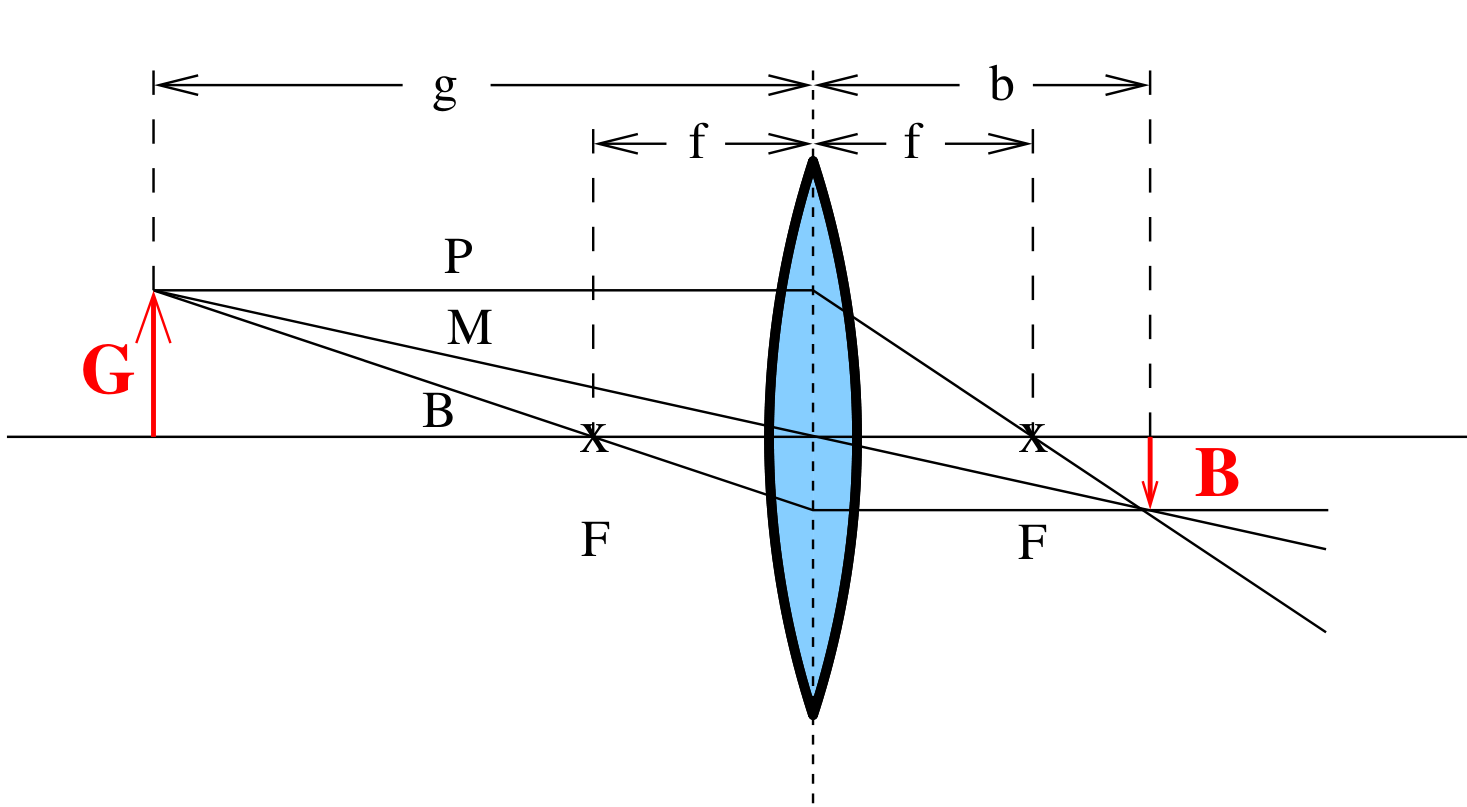
\includegraphics[width = 0.7\textwidth]{Pics/Sammellinse.png}
  \caption{Bildrekonstruktion des Strahlenverlaufs bei einer Sammellinse.\cite{anleitung01}}
  \label{fig:Sammellinse}
\end{figure}

Ein weiterer Typus ist die Streulinse, bei der die Lichtstrahlen vom Einfallslot
weg gebrochen werden. Dadurch entsteht lediglich ein virtuelles Bild, welches
eine negative Bildweite besitzt (siehe Abbildung \ref{fig:Streulinse}). Aufgrund dieser
Eigenschaften wird bei Sammellinsen von einer positiven Brennweite und bei
Streulinsen von einer negativen Brennweite gesprochen.

\begin{figure}
  \centering
  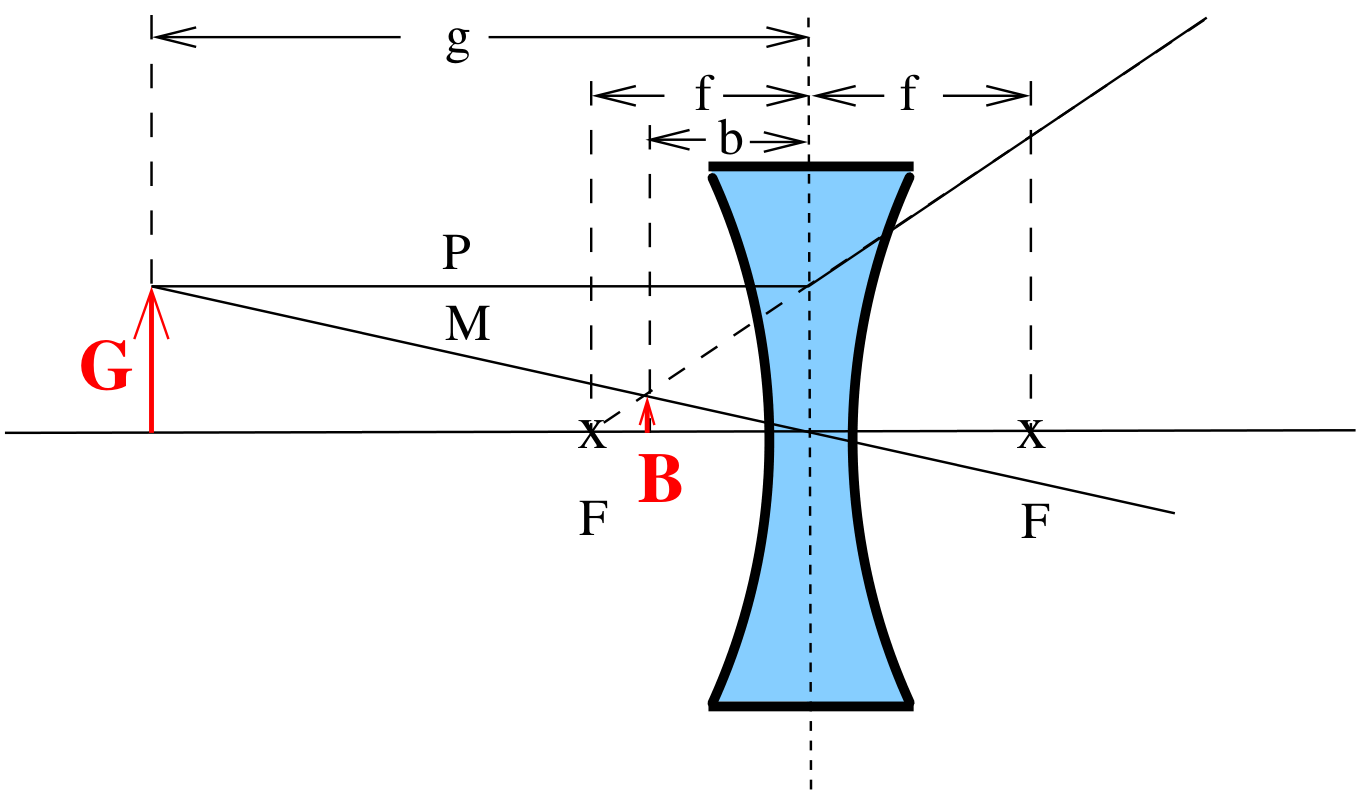
\includegraphics[width = 0.7\textwidth]{Pics/Streulinse.png}
  \caption{Bildrekonstruktion bei einer Streulinse. \cite{anleitung01}}
  \label{fig:Streulinse}
\end{figure}

Während bei einer dünnen Linse die Brechung auf lediglich eine Mittelenbene reduziert
werden kann, müssen bei dickeren Linsen zwei Hauptebenen betrachtet werden (siehe
Abbildung \ref{fig:dickeLinse}). Um nun optische Bildrekonstruktionen durchzführen, werden
drei charakteristische Strahlen eingeführt.

\begin{itemize}
  \item \underline{Parallelstrahl}: Der Parallelstrahl läuft von der Gegenstand
  senkrecht auf die Mittel- bzw. Hauptebene zu, wird dort gebrochen und läuft
  dann durch den Brennpunkt.
  \item \underline{Mittelpunktsstrahl}: Der Mittelpunktsstrahl läuft direkt durch
  die Mitte der Linse und läuft durchgehen in die selbe Richtung.
  \item \underline{Brennpunktstrahl}: Der Brennpunktstrahl läuft durch den Brennpunkt
  auf die Mittel- bzw.  Haupteben zu, wird dort gebrochen und läuft dann senkrecht
  zur Mittel- bzw. Hauptebene bis zum Bild.
\end{itemize}

\begin{figure}
  \centering
  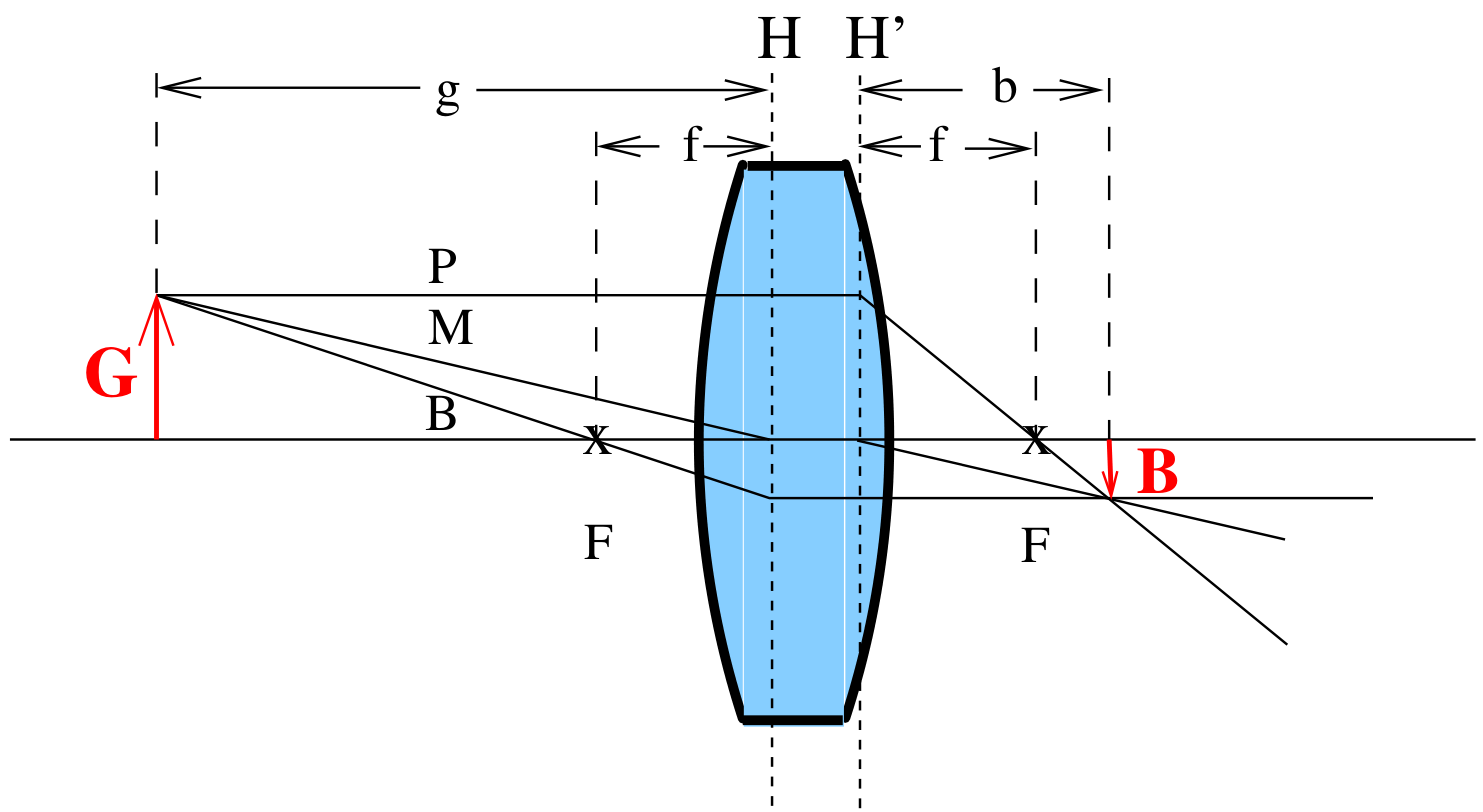
\includegraphics[width = 0.7\textwidth]{Pics/dickeLinse.png}
  \caption{Darstellung der Bildrekonstruktion bei einer dicken Linse.\cite{anleitung01}}
  \label{fig:dickeLinse}
\end{figure}

Der Schnittpunkt aller drei Strahlen markiert dann das Abbild. Zwischen den, bei der
Bildrekonstruktion betrachteten Größen besteht nach dem Abbildungsgesetz folgender
Zusammenhang:

\begin{equation}
  V = \frac{B}{G} = \frac{b}{g},
  \label{eqn:Abbildungsgesetz}
\end{equation}

wobei V den Abbildungsmaßstab, B und G Bild- bzw. Gegenstandsgröße und b und g die
Bild- bzw. Gegenstandsweite beschreiben. Für dünne Linsen folgt zudem die Linsengleichung,
welche eine Zusammenhang zwischen der Brennweite f sowie b und g herstellt (Formel
\eqref{eqn:Linsengleichung}).

\begin{equation}
\frac{1}{f} = \frac{1}{b} + \frac{1}{g}
\label{eqn:Linsengleichung}
\end{equation}

Bei dickeren Linsen müssen zwei Hauptebenen betrachtet
werden. Hier werden Brennweite und weitere Größen immer bezüglich einer Hauptebene
angegeben, sodass die Linsengleichung auch hier ihre Gültigkeit behält.

Durch Linsen erzeugte Abbildungen können aufgrund der Gültigkeit der Formeln
\eqref{eqn:Abbildungsgesetz} und \eqref{eqn:Linsengleichung} für achsennahe Strahlen
einen Abbildungsfehler bei der Betrachtung achsenferner Strahlen haben.
Bei der sphärischen Abberration liegen die Brennpunkte beider Strahlentypen nicht
aufeinander, sodass es zu einer Unschärfe kommt. Dieser Fehler kann allerdings
durch eine Irisblende behoben werden. Bei der chromatischen Abberation kommt es
aufgrund der unterschiedlichen Wellenlängen im Lichtspektrum zu einer Dispersion
bei der Brechung verschiedener Farben.

Eine weitere Größe zur Beschreibung von Linsen ist die Brechkraft D, welche als
reziproke Brennweite definiert ist. Bei einem System von mehreren dünnen Linsen
können die einzelnen Brechkräfte einfach summiert werden:

\begin{equation}
  D = \sum_{i}^{N} D\ua{i} = \sum_{i}^{N} \frac{1}{f\ua{i}} .
\end{equation}

Zur Bestimmung der Brennweite einer Linse werden im Folgendem mehrere Methoden erläutert.
Erstens kann die Brennweite durch Messung von Bild- und Gegenstandsweite bestimmt
werden. Dafür wird die Linsengleichung (Formel \eqref{eqn:Linsengleichung}) genutzt,
um aus Bild- und Gegenstandsweite die Brennweite zu bestimmen (siehe Abb.
\ref{fig:Sammellinse}).


Eine weitere Möglickeit bietet die Methode nach Bessel. Hier wird der Abstand zwischen
Gegenstand und Bild konstant gehalten und es werden zwei verschiedene Positionen
gesucht, bei denen das Bild scharf dargestellt wird (siehe Abbildung \ref{fig:2Sammellinsen}).
Da es sich um eine symmetrische Linsenstellung handelt, gilt folgende Beziehung:

\begin{equation}
  b\ua{1} = g\ua{2} \,\, \su{und} \,\, b\ua{2} = g\ua{1} .
\end{equation}

Mit den Größen $e = g\ua{1} + b\ua{1} = g\ua{2} + b\ua{2}$ (Abstand zwischen Bild
und Gegenstand) sowie $d = g\ua{1} - b\ua{1} = g\ua{2} - b\ua{2}$ (Abstand zwischen
den beiden Linsenpositionen) lässt sich dann ein Formel für die Brennweite der
Linse herleiten (Formel \eqref{eqn:Bessel}).

\begin{equation}
  f = \frac{e^2 - d^2}{4e}
  \label{eqn:Bessel}
\end{equation}

\begin{figure}
  \centering
  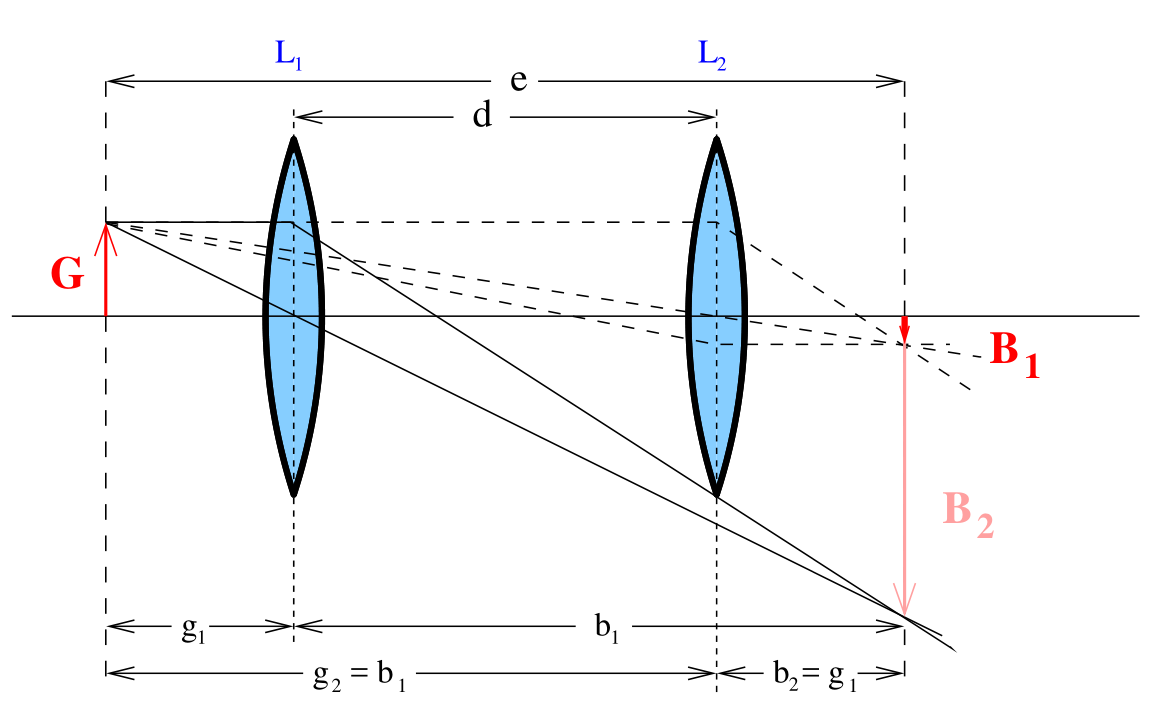
\includegraphics[width = 0.7\textwidth]{Pics/2Sammellinsen.png}
  \caption{Linsenpositionen zur Bestimmung der Brennweite mit der Methode von Bessel.\cite{anleitung01}}
  \label{fig:2Sammellinsen}
\end{figure}

Eine weitere Methode zur Bestimmung der Brennweite ist die Methode von Abbe. Bei
dieser können Brennweite und Lage der Hauptebenen aus dem Abbildungsmaßstab hergeleitet
werden. Dafür werden bei einer dicken Linse wieder Bild- und Gegenstandsweite in
Bezug zu einem beliebigen Bezugspunkt A gemessen (siehe Abb. \ref{fig:Linsensystem}).
Hierbei gelten folgende Beziehungen:

\begin{align}
  \label{eqn:Abbe1}
  g´ &= g + h  = f \cdot \left( 1 + \frac{1}{v} \right) +h \\
  \label{eqn:Abbe2}
  b´ &= b + h´ = f \cdot \left( 1 + v \right) + h´ .
\end{align}

\begin{figure}
  \centering
  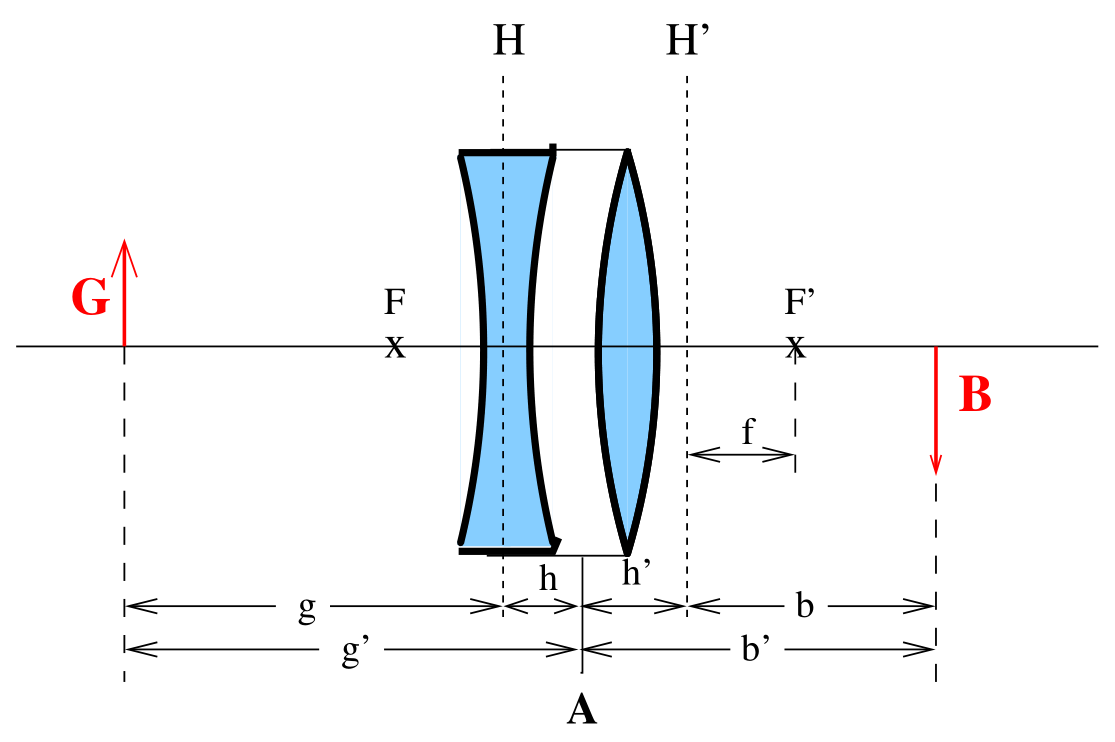
\includegraphics[width = 0.7\textwidth]{Pics/Linsensystem.png}
  \caption{Aufbau des Linsensystems bei der Bestimmung der Brennweite mittels der
  Methode von Abbe.\cite{anleitung01}}
  \label{fig:Linsensystem}
\end{figure}

Der gewählte Referenzpunkt A muss dabei nicht innerhalb der Hauptebenen liegen.

\section{Versuchsaufbau und Durchführung}

Es wird ein Aufbau nach Abbildung \ref{fig:Aufbau} verwendet. Auf einer
Schiene werden die verwendete Blende mit L-förmig angeordneten punktförmigen
Spalten (2), die verschiedenen Linsen (3) sowie der Schirm (4) montiert. Die als
Lichtquelle verwendete Halogenlampe (1) wird vor der Schiene aufgestellt.
Mit der auf der Schiene vorhandenen Längenskala werden die verschiedenen
Abstände gemessen.

\begin{figure}
  \centering
  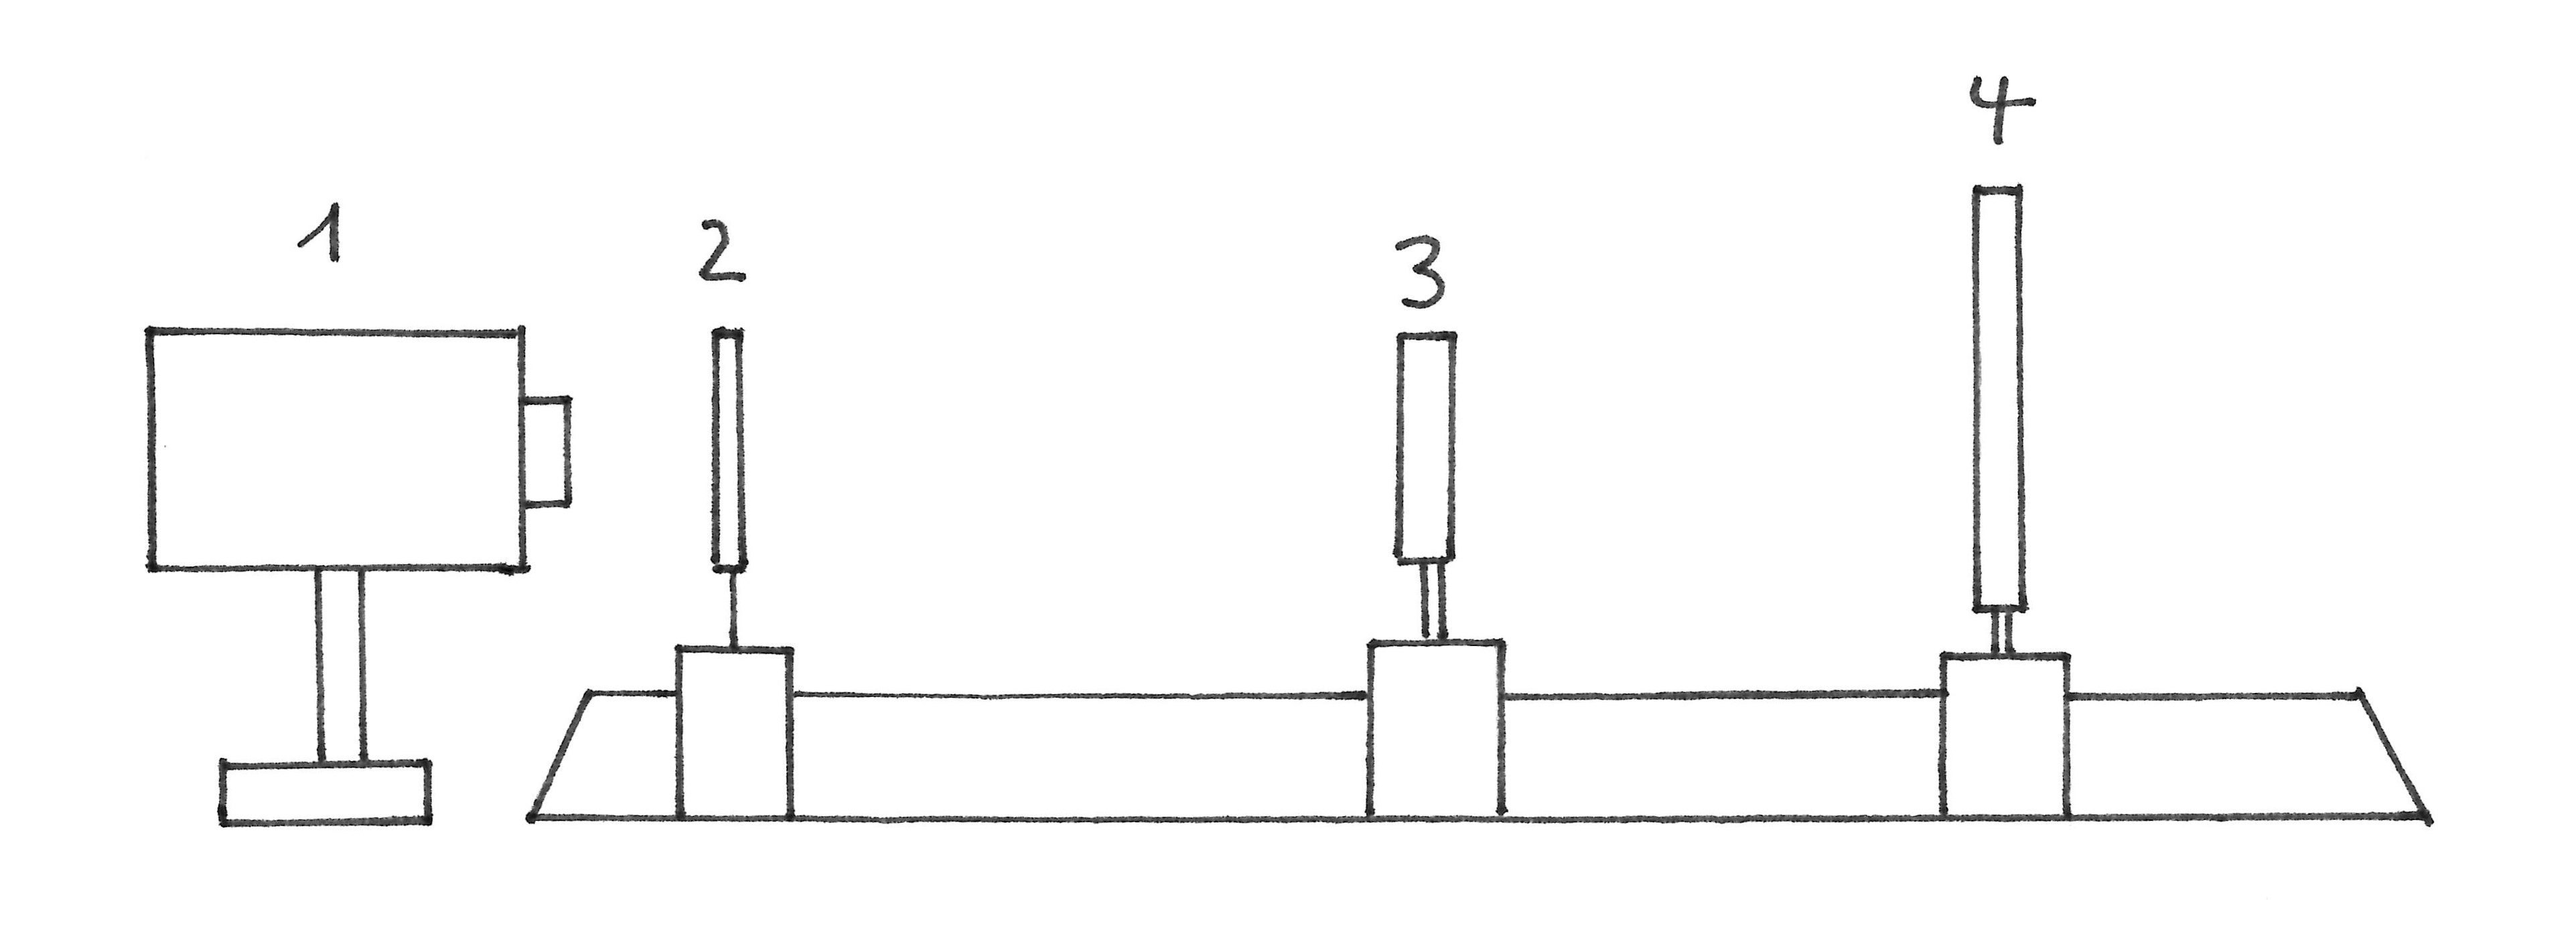
\includegraphics[width = 0.7\textwidth]{Pics/Aufbau.JPG}
  \caption{Schematische Darstellung des verwendeten Aufbaus bei den folgenden Messungen. \cite{anleitung01}}
  \label{fig:Aufbau}
\end{figure}

\subsection{Bestimmung der Brennweite durch Messung der Bild- und Gegenstandsweite}

Zuerst wird eine Sammellinse mit bekannter Brennweite auf der Schiene montiert.
Mit der Linse und der
Längenskala werden dann verschiedene Gegenstandsweiten eingestellt. Durch
Verschieben des Schirmes zu einem Punkt, auf dem das Bild scharf erscheint
werden die entsprechendem Bildweiten gemessen. Diese Messung wird 10 mal für
verschiedene Gegenstandsweiten durchgeführt.
Bei den ersten fünf Messungen werden zudem Bild- und Gegenstandsgröße gemessen.

Anschließend wird eine dehnbare, mit Wasser gefüllte Linse auf der Schiene montiert.
Während mit dem selben Verfahren wie bei der Sammellinse die Gegenstand- und Bildweite
gemessen werden, wird mit einer Spritze ein konstanter Druck innerhalb der
Linse aufrecht erhalten. Auch diese Messung wird 10 mal für verschiedene
Gegenstandsweiten durchgeführt.

Danach wird mit der Linse noch einmal die Akkomodation des Auges betrachtet, indem
bei konstanter Bild- und Gegenstandsweite der Druck in der Linse solange verändert
wird, bis das Bild auf dem Schirm scharf erscheint.

\subsection{Bestimmung der Brennweite mit der Methode von Bessel}

Zuerst werden Blende und Schirm auf einen konstanten Abstand gebracht. Nun
wird die Sammellinse zwischen Schirm und Blende verschoben, bis auf dem Schirm
ein scharfes Bild zu sehen ist. Das dadurch entstehende Wertepaar aus Bild-
und Gegenstandsweite wird notiert. Danach wird die Linse bei konstantem Abstand
zwischen Schirm und Blende noch weiter verschoben, bis das Bild erneut scharf
dargestellt wird. Das zweite Wertepaar wird ebenfalls notiert. Die Messung
wird 10 mal für verschiedene Abstände zwischen Blende und Schirm durchgeführt.

Um die chromatische Abberation betrachten zu können, werden
anschließend nacheinander ein roter und ein blauer Filter vor die
Blende montiert. Für beide Filter wird die Messung nach der Besselmethode
fünf mal durchgeführt.

\subsection{Bestimmung der Brennweite mit der Methode von Abbe}

Die Methode nach Abbe beschäftigt sich mit der Brennweitenbestimmung von Linsensystemen.
Zuerst wird ein Linsensystem aus Streu- und Sammellinse auf
dem Schirm montiert. Dabei werden die Reiter beider Linsen direkt aneinander
geschoben und der Berührungspunkt wird als Referenzpunkt A gewählt. Nun wird
mithilfe des Systems eine bestimmte Gegenstandsweite eingestellt. Der Schirm wird
solange verschoben, bis das Bild scharf erscheint. Das entstehende Wertepaar aus
Bild- und Gegenstandsweite, sowie die Bildgröße werden notiert und die Messung
anschließend neun mal für verschiedene Gegenstandsweiten wiederholt.
